
\chapter{Method}\label{ch:methodology}

This chapter specifies the system in the order a query passes through
it. Section~\ref{sec:arch-requirements} states what a partition has to
satisfy for a per-cell arena to mean anything, and
Section~\ref{sec:arch-taxonomy} gives the construction that produces
one, ending with the frozen artifact every result is attributed to.
Section~\ref{sec:arch-arena} specifies the arena: what it judges, what
the judge sees, how comparisons are scheduled, and how verdicts become
per-cell and per-domain rankings. Section~\ref{sec:meth-validation}
gives the two statistics the rankings are validated against.
Section~\ref{sec:meth-assumptions} and
Section~\ref{sec:meth-discipline} state what the method assumes and the
reporting rules it holds itself to. Section~\ref{sec:arch-infra} closes
the chapter with what the run seed fixes and what ``reproducible''
means here.

Figure~\ref{fig:pipeline} is the whole path on one page. Everything
after it fills in a box.

One term recurs throughout and is easier to define once. Before any
construction happens the corpus is cut in two. Seventy per cent becomes
the \emph{construction pool}; the remaining thirty per cent is
\emph{reserved}, and those are the only queries the arena is ever
allowed to judge. The tree is built from the construction pool alone,
and each leaf's rubric is written from the construction pool alone. A
reserved query is first touched when it is routed into a cell at
judging time, and its correct answer is not read until every verdict
has been recorded. \emph{Held-out query} means a member of that
reserved pool.
The separation is what the evaluation rests on. If a leaf's rubric had
been written from the questions that leaf is later asked to grade, a
judge following the rubric could be recognising a question rather than
assessing an answer, and no comparison against the answer key would
mean anything. The split, the filter that enforces it, and the
build-time assertion that audits the filter are
Section~\ref{sec:exp-info-separation} and Section~\ref{sec:arch-judge}.

\usetikzlibrary{positioning}

\begin{figure}[htbp]
\centering
\footnotesize
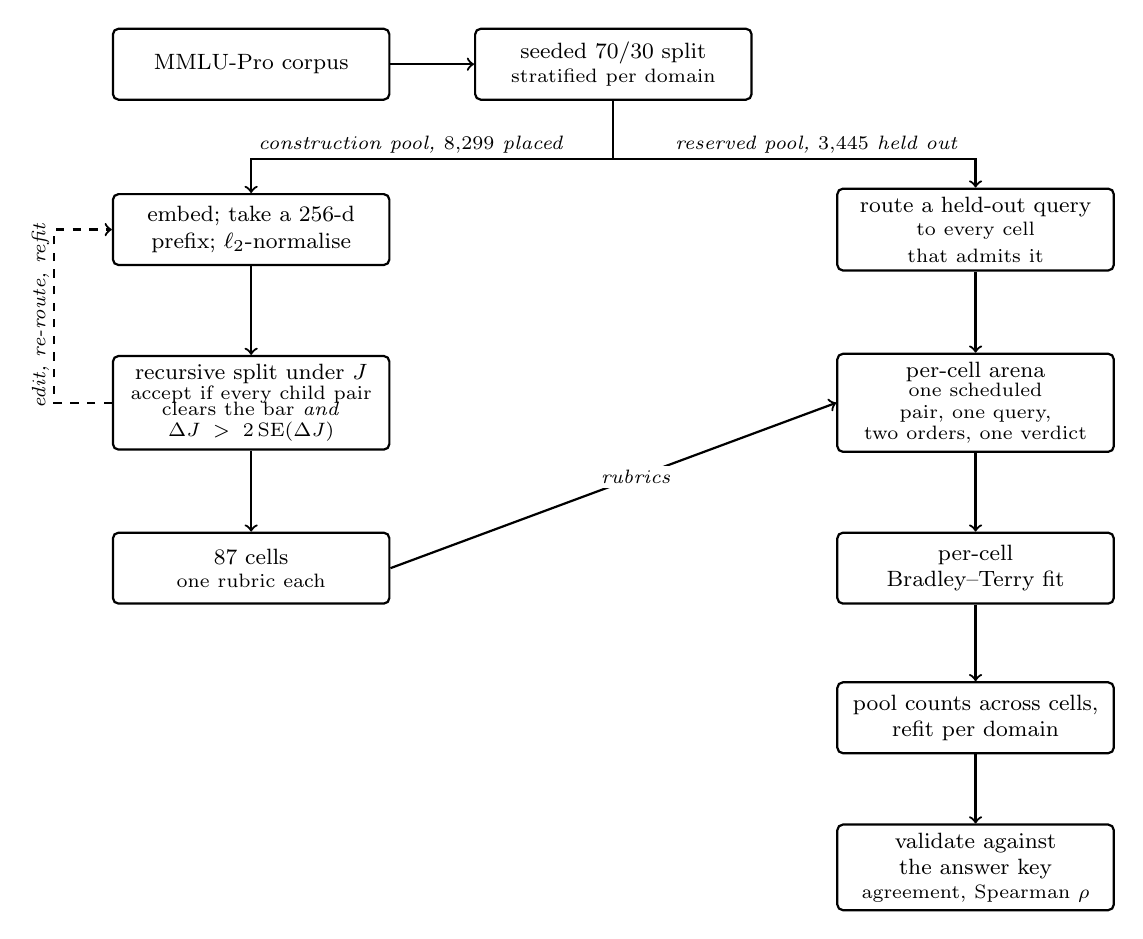
\begin{tikzpicture}[
  x=1cm, y=1cm,
  box/.style={draw, rounded corners=2pt, align=center, inner sep=3pt,
              minimum height=9mm, text width=33mm, font=\footnotesize},
  lab/.style={font=\scriptsize\itshape, align=center, inner sep=1.5pt},
  ->, thick
]

% ── the split ────────────────────────────────────────────────────────
\node[box] (corpus) at (0,0)   {MMLU-Pro corpus};
\node[box] (split)  at (4.6,0) {seeded $70/30$ split\\[-1pt]
                                 \scriptsize stratified per domain};
\draw (corpus) -- (split);

% ── construction lane (left) ─────────────────────────────────────────
\node[box] (embed) at (0,-2.1) {embed; take a 256-d\\prefix; $\ell_2$-normalise};
\node[box] (rec)   at (0,-4.3) {recursive split under $J$\\[-1pt]
                                 \scriptsize accept if every child pair\\[-2pt]
                                 \scriptsize clears the bar \emph{and}\\[-2pt]
                                 \scriptsize $\Delta J > 2\,\mathrm{SE}(\Delta J)$};
\node[box] (cells) at (0,-6.4) {87 cells\\[-1pt]\scriptsize one rubric each};

% ── arena lane (right) ───────────────────────────────────────────────
\node[box] (route) at (9.2,-2.1) {route a held-out query\\[-1pt]
                                   \scriptsize to every cell that admits it};
\node[box] (arena) at (9.2,-4.3) {per-cell arena\\[-1pt]
                                   \scriptsize one scheduled pair, one query,\\[-2pt]
                                   \scriptsize two orders, one verdict};
\node[box] (fit)   at (9.2,-6.4) {per-cell\\Bradley--Terry fit};
\node[box] (pool)  at (9.2,-8.3) {pool counts across cells,\\refit per domain};
\node[box] (valid) at (9.2,-10.2){validate against the answer key\\[-1pt]
                                   \scriptsize agreement, Spearman $\rho$};

% ── branch from the split ────────────────────────────────────────────
\draw (split.south) -- (4.6,-1.2) -| node[lab, pos=0.28, above]
      {construction pool, $8{,}299$ placed} (embed.north);
\draw (split.south) -- (4.6,-1.2) -| node[lab, pos=0.28, above]
      {reserved pool, $3{,}445$ held out} (route.north);

% ── lane flows ───────────────────────────────────────────────────────
\draw (embed) -- (rec);
\draw (rec) -- (cells);
\draw (route) -- (arena);
\draw (arena) -- (fit);
\draw (fit) -- (pool);
\draw (pool) -- (valid);

% ── the one cross-link: cells supply the rubrics ─────────────────────
\draw (cells.east) -- node[lab, fill=white, pos=0.55] {rubrics} (arena.west);

% ── the construction loop ────────────────────────────────────────────
\draw[dashed] (rec.west) -- (-2.5,-4.3) -- (-2.5,-2.1)
      node[lab, midway, left, rotate=90, anchor=south]
      {edit, re-route, refit} -- (embed.west);

\end{tikzpicture}
\caption[The pipeline from corpus to validated ranking]{The path a
query takes. The corpus is split $70/30$ once, under the run's seed
($8{,}673 + 3{,}445$); construction sees only the left lane and
produces 87 cells with one rubric each, the arena judges only the
right lane, and the dashed arrow is the construction loop (edit,
re-route, refit, until neither moves)}
\label{fig:pipeline}
\end{figure}

Three different totals appear in the artifacts, and only one of them is
the corpus.

MMLU-Pro supplies $12{,}118$ questions that carry evaluation rows for
this roster. The seeded $70/30$ split sends $8{,}673$ to construction and
holds out $3{,}445$; those two sum to the corpus exactly. Of the
construction share, $8{,}299$ are placed in the tree --- the snapshot's
own \texttt{totalUniqueQueries} --- and the remaining $374$ are dropped
during routing as outliers. The embedding cache holds $11{,}773$ vectors,
$345$ short of the corpus; the missing questions had no usable
embedding.

Question identifiers here are \texttt{eval\_results.question\_id}, not
\texttt{mmlu\_pro.id}. The two occupy different spaces and resolve to
different questions for the same integer, so the $12{,}118$ above is not
comparable with the $12{,}000$ items MMLU-Pro is usually quoted as
holding (Appendix~\ref{app:models}).

\section{What a Good Partition Needs}\label{sec:arch-requirements}

The design is betting on one thing, and the requirements below are
conditions for that bet to be testable rather than the bet itself. The
bet is that two queries whose embeddings point in nearly the same
direction are asking for the same kind of work: the same concepts, the
same methods, the same characteristic ways of going wrong. If that
holds, a cell is a group of queries a model tends to succeed or fail on
together, a rubric can be written that is true of the whole cell and
still specific enough to discriminate, and a per-cell ranking becomes a
statement about a capability rather than about a topic label. Whether
cell-scoped judging actually produces better judgments is links~2 and~3
of Section~\ref{sec:research-questions}, and the answer is
Chapter~\ref{ch:results}.

Four requirements follow. They are stated before any construction
detail so the construction can be assessed against them.

\begin{description}
\item[R1 --- Coherence.] Cells must be homogeneous enough that a single
rubric fits every query in the cell. This is the requirement the whole
design exists to serve (Section~\ref{sec:problem-statement}).
\item[R2 --- Support.] Cells must be large enough that per-cell judging
is identifiable --- the comparison graph connects --- and that per-cell
reliability is not dominated by sampling noise.
\item[R3 --- Stability.] The same corpus \emph{and the same seed} must
yield the same cells, and the construction must reach a state that one
further application of its own operator would not change. The seed
clause is not decorative: leaf counts and leaf boundaries move across
seeds, and Section~\ref{sec:res-construction} reports by how much.
\item[R4 --- Verifiability.] The construction's guarantees and its
non-guarantees must be enumerable, and fixed before any result depends
on them.
\end{description}

Whether the construction meets R1--R4 is an empirical question.
Section~\ref{sec:res-construction} collects one line of evidence per
requirement, each with the caveat that bounds it.

\section{Building the Partition}\label{sec:arch-taxonomy}

The 14 MMLU-Pro domain labels seed 14 immutable top-level anchor nodes.
They are held immutable so that every induced cell stays nested under
one MMLU-Pro top-level domain, which is what allows a per-domain result
to be set against MMLU-Pro's own published category scores.

Every corpus query is embedded, and a fixed 256-dimensional prefix
slice of the embedding is $\ell_2$-normalised to the unit hypersphere
and used at every depth. Truncation is safe only because
Qwen3-Embedding-8B is trained under Matryoshka Representation
Learning \parencite{kusupati2022mrl}, so every prefix is itself a
usable embedding. The construction needs the fixed narrow width for
two reasons: it keeps the directional concentration estimates well
conditioned at these cell sizes, and one width at every depth puts
all nodes on the same sphere, comparable without projecting between
spaces. All $11{,}773$ embeddings are retained at full native width,
so the tree can be rebuilt without re-contacting the model (which was
served under a moving tag); the width of $256$ is a fixed operating
point this thesis does not ablate, and
Appendix~\ref{sec:meth-mrl} states both the argument for it and why
an ablation would not isolate what it appears to.

Queries then migrate by embedding geometry, so a query labelled
Mathematics may come to sit under a different anchor. This is what
makes the induced (\textit{adapted}) partition differ from the
editorial (\textit{canonical}) one.

\subsection{The Acceptance Test}\label{sec:arch-acceptance}

Each anchor is recursively split under a chance-corrected separation
score $J$. Chance-corrected means measured against what the same split
would score by chance, so the threshold does not drift with cell size:
$J$ measures how much better the observed split separates the queries
than the same queries randomly relabelled into clusters of the same
sizes, and a high $J$ therefore cannot be produced by the cell-size
structure alone. The formal definition is in
Appendix~\ref{app:dag-formalism}. Candidate splits are proposed in a
size-dependent principal-component subspace of 32, 64 or 128
dimensions, and every acceptance gate is evaluated in the full
256-dimensional routed space, so the subspace shapes the candidates and
never the decision.

A split is accepted when two conditions hold together, shown in
Figure~\ref{fig:acceptance}. Every child pair must clear a separation
bar of $0.025$, and the improvement $\Delta J$ the split buys must
exceed twice its own paired bootstrap standard error. The second
condition is what makes the gate scale-free. $\mathrm{SE}(\Delta J)$
varies by more than an order of magnitude across sites on this corpus,
so a fixed threshold on $\Delta J$ would be strict at one site and
permissive at another; expressing the gate in standard-error units
removes that.

Two fallbacks complete the rule and both matter downstream. Where the
paired standard error is zero, the edit is accepted if it strictly
reduces the node count, which is how pass-through wrappers dissolve. A
hard tolerance floor $\tau = 10^{-6}$ applies underneath, which is what
makes the termination bound finite. On the frozen run that floor never
bound: the smallest threshold any decision was taken against is
$88\tau$, so what governed every acceptance was the standard error.

\begin{figure}[htbp]
\centering
\footnotesize
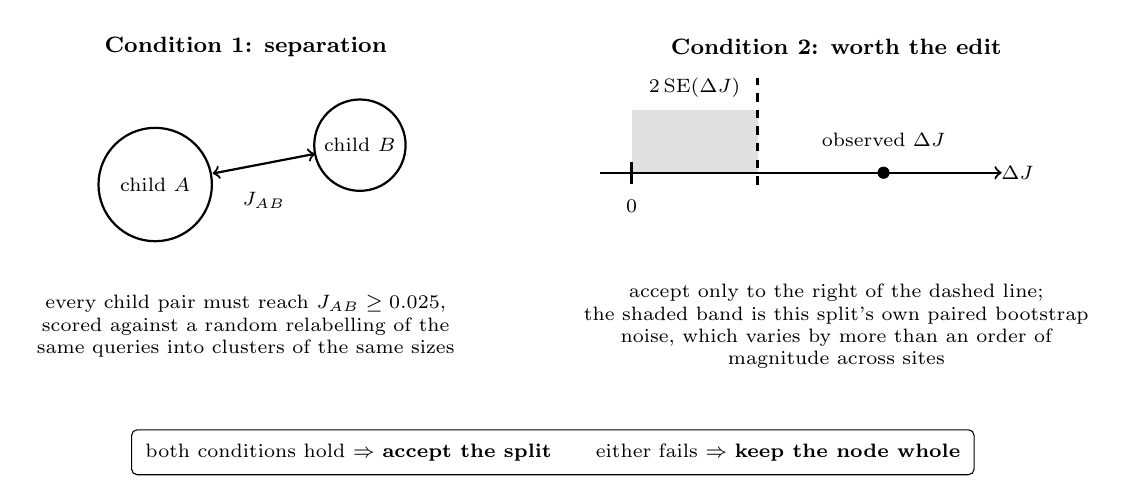
\begin{tikzpicture}[
  x=1cm, y=1cm,
  every node/.style={align=center},
  note/.style={font=\scriptsize, align=center}
]

% ── left panel: separation between the proposed children ────────────
\node[font=\footnotesize\bfseries] at (1.7,3.3) {Condition 1: separation};
\draw[thick] (0.55,1.55) circle (0.72);
\draw[thick] (3.15,2.05) circle (0.58);
\node[font=\scriptsize] at (0.55,1.55) {child $A$};
\node[font=\scriptsize] at (3.15,2.05) {child $B$};
\draw[<->, thick] (1.28,1.69) -- (2.58,1.94);
\node[font=\scriptsize] at (1.93,1.35) {$J_{AB}$};
\node[note] at (1.7,-0.25)
  {every child pair must reach $J_{AB} \geq 0.025$,\\
   scored against a random relabelling of the\\
   same queries into clusters of the same sizes};

% ── right panel: the delta-J test ───────────────────────────────────
\node[font=\footnotesize\bfseries] at (9.2,3.3) {Condition 2: worth the edit};
\fill[black!12] (6.6,1.7) rectangle (8.2,2.5);
\draw[thick, dashed] (8.2,1.55) -- (8.2,2.9);
\node[font=\scriptsize] at (7.4,2.78) {$2\,\mathrm{SE}(\Delta J)$};
\draw[thick, ->] (6.2,1.7) -- (11.3,1.7);
\node[font=\scriptsize] at (11.5,1.7) {$\Delta J$};
\draw[thick] (6.6,1.56) -- (6.6,1.84);
\node[font=\scriptsize] at (6.6,1.28) {$0$};
\fill (9.8,1.7) circle (2.2pt);
\node[font=\scriptsize] at (9.8,2.12) {observed $\Delta J$};
\node[note] at (9.2,-0.25)
  {accept only to the right of the dashed line;\\
   the shaded band is this split's own paired bootstrap\\
   noise, which varies by more than an order of\\
   magnitude across sites};

% ── verdict ─────────────────────────────────────────────────────────
\node[draw, rounded corners=2pt, inner sep=5pt, font=\scriptsize]
  at (5.6,-1.85)
  {both conditions hold $\Rightarrow$ \textbf{accept the split}\quad\quad
   either fails $\Rightarrow$ \textbf{keep the node whole}};

\end{tikzpicture}
\caption[What the acceptance test compares]{One accept/reject
decision: a split must clear a separation condition (children far
enough apart on the sphere) and a noise condition (the gain in $J$
larger than its own standard error). Both are evaluated in the full
256-dimensional space, whatever subspace proposed the candidate}
\label{fig:acceptance}
\end{figure}

Four coarsening moves run in the same loop --- absorption of
below-floor children, merging of insufficiently separated siblings,
merging of redundant nodes, and dissolution of pass-through nodes ---
so every operator maps a tree to a tree. Only the last of the four
accepted anything in this artifact, twice, and no fusion of any kind
ever fired; the loop is symmetric by construction and asymmetric in
use. The loop runs until one of two stopping criteria fires, and both
are given in limitation~3 below. The formalism, the parameter
derivations, the routing rule and the certificate are given in full in
Appendix~\ref{app:dag-formalism} and Appendix~\ref{app:numerics}; how
the parameters were arrived at is Appendix~\ref{app:tuning-protocol}.

\subsection{The Frozen Artifact}\label{sec:arch-frozen}

Every construction and arena result in this thesis is attributed to one
snapshot. Table~\ref{tab:frozen-artifact} states it.

\begin{table}[htbp]
    \centering
    \caption[The frozen construction artifact]{The frozen construction
    artifact. Every configuration value is the one recorded in the
    snapshot's stored settings and echoed on the
    \texttt{Loaded CLI Configuration} line of every arena run log.}
    \label{tab:frozen-artifact}
    \small
    \begin{tabular}{ll}
        \toprule
        Snapshot & \texttt{20260727\_042523\_}\\
                 & \texttt{Headless\_Run\_Auto\_ge} \\
        Configuration & \texttt{experiment\_configs/}\\
                      & \texttt{freeze\_mcs55.toml} \\
        Seed & $42$ \\
        Split & \texttt{testRatio} $=0.3$, stratified within each domain \\
        \addlinespace
        Nodes / cells / depth & $154$ / $87$ / $6$ \\
        Construction queries placed & $8{,}299$ of $8{,}673$ \\
        Reserved (held-out) queries & $3{,}445$ \\
        Separation score $J$ & $0.253129$ \\
        Labels and rubrics & $87/87$ cells carry both \\
        \addlinespace
        \texttt{minClusterSize} & $55$ \\
        \texttt{proposalSeparationBar} & $0.025$ \\
        \texttt{acceptanceZ} & $2.0$ \\
        $\tau$ (and the separate $\theta$ tolerance) & $10^{-6}$ \\
        \texttt{maxDepth} (cap; realised depth $6$) & $8$ \\
        \texttt{maxLeafAssignments} & $5$ \\
        \bottomrule
    \end{tabular}
\end{table}

Of the $154$ nodes, $87$ are leaves and carry queries, rubrics and
labels; the other $67$ are internal nodes, which include the root and
the 14 domain anchors and carry no rubric. ``87 cells'' and ``154
nodes'' describe the same tree. Where this thesis says \emph{cell} it
means one of the 87 leaves.

\texttt{minClusterSize} $=55$ is a budget choice rather than a
statistical requirement. It was set so that the cell count matches what
the judge budget can identify, and the resulting per-cell reliability
follows from it. What licenses treating it as free is a measured
result: discriminative power is flat from 14 to 152 cells
(Section~\ref{sec:res-granularity}), so the cell count can be chosen on
cost grounds at no evaluative cost.

The fixed-point certificate is a four-term tolerance test asking
whether one further application of the construction operator would
change the frozen artifact. All four terms are magnitudes rather than
counts: the edit-phase change in $J$, the re-routing change in $J$, and
the maximum per-node change in direction and in concentration. The two
objective terms are tested against $\tau$; the two parameter terms are
tested against a separate tolerance on $\theta$, because $\tau$ bounds
a change in $J$ and these bound a change in the parameters that produce
it. Both tolerances are $10^{-6}$, which is a coincidence of value and
not of meaning. The parameter terms are the reason the certificate
exists at all: a held-out query is routed through $\theta$, so a check
over structure and objective alone would not cover the object being
frozen. The certificate's realised values are reported with the results
(Section~\ref{sec:res-construction}).

\subsection{Four Things the Construction Does Not Guarantee}\label{sec:arch-limits}

These are stated here, before Chapter~\ref{ch:results}.

\begin{enumerate}
\item \textbf{``Chance-corrected'' means corrected against relabelling,
not against anisotropy.} What $J$ corrects for is how well a split of
the same size profile would separate the queries if its labels had been
assigned at random. One failure survives that correction. Consider a
node whose queries form a single elongated cluster, cut in half across
its own long axis. The two halves are one topic, but they sit far
enough apart to beat a random relabelling, so $J$ scores the cut as a
real split. A subset of accepted splits therefore cannot be
distinguished from such a cut on the evidence $J$ provides. The counts
that quantified this exposure are \textsc{void as to values} (marker
defined in Section~\ref{sec:res-construction}) and are not restated.
One bound survives the voiding. The separation bar sits $2.7$ to $4.5$
times above the isotropic null's $p_{95}$ and below the median of the
within-node null, so it is conservative against ``separated at all''
and permissive against ``separated by more than this node's own
elongation''; the one node that reached that boundary in the frozen run
was declined.

\item \textbf{The size floor is a birth constraint.} It is enforced on
the routed partition at split time. Populations drift as later
iterations re-route queries, so about one cell in a hundred ends
marginally below it --- 1 of 87 in this artifact, with two further
consistent instances at other settings. The below-floor cell is visible
at the left edge of the cell-size distribution
(Figure~\ref{fig:leaf-size-hist}). Any statement of the form ``every
cell holds at least \texttt{minClusterSize} queries'' is false as
written. This is a property of the mechanism, not a defect.

\item \textbf{The loop can stop for either of two reasons, and the
weaker one is what stopped it.} A \emph{structural} criterion (five
consecutive iterations at graph edit distance zero, with a floor of
11 iterations at fourteen anchors) and an \emph{objective} criterion
($J$ stationary within $\tau$ for five consecutive iterations) each
end the run. The frozen run stopped at iteration~10 on the objective
criterion, below the structural floor, so a tree that keeps
rearranging itself without moving $J$ satisfies the criterion that
actually stopped this run. The fixed-point certificate is a separate,
period-1 check; Appendix~\ref{subsec:quiescence} details both
criteria and the seed runs that stop in a period-2 cycle neither can
see (Section~\ref{sec:res-construction} reports them).

\item \textbf{Nothing here guarantees that a held-out query reaches the
right cell.} Every arena result depends on cell membership for queries
the construction never saw, and that membership is produced by soft
routing rather than by the construction. A held-out query is scored
against every cell, the cells are ranked by posterior, and at most
$\texttt{maxLeafAssignments} = 5$ are kept --- one primary and up to
four secondaries --- with an entropy guard that drops all secondaries
when the posterior over cells is close to uniform. The $0.25$
membership floor named in the configuration governs construction-time
trickling and is not a threshold on this admission step. The one
exported measure of routing quality, expected calibration error at
$0.2114$, is computed under a defective aggregation that understates
every confidence (Appendix~\ref{app:metrics}), so its value is a
diagnostic and not a bound. No result in this thesis validates held-out
routing directly.
\end{enumerate}

None of R1--R4 tests the bet stated at the head of
Section~\ref{sec:arch-requirements}. R1 and R2 say only that the arena
can be run inside these cells and that its per-cell estimates are
identified; R3 and R4 say that the object being run inside is fixed and
described.


%% ---- (was 4_Methodology.tex; merged 2026-07-31) ----

\section{The Arena}\label{sec:arch-arena}

\subsection{What the Arena Is}\label{sec:arch-overview}

\textbf{The arena does not query models.} It re-judges responses that
were generated and stored earlier, in an evaluation corpus that also
records each model's selected answer. A run consists of routing
held-out queries through a frozen snapshot, retrieving two stored
responses per comparison, and issuing judge calls. No response is
produced during a run.

The responses were not generated for this thesis either. They come from
the per-model evaluation archives the MMLU-Pro authors publish
alongside the corpus \parencite{wang2024mmlupro}, one archive per
model, each holding that model's selected option and, for most models,
the reasoning text it produced. Ingestion is one archive at a time, and
each one has to pass a consensus check on question identity before the
model is admitted to a run; that check and the exclusions it enforces
are Section~\ref{sec:exp-rosters} and Appendix~\ref{app:models}.

This is stated first because two later results are unintelligible
without it. First, a model whose response text was never persisted
cannot be distinguished downstream from one whose text was. The trace
accessor never returns an empty string, and synthesises a one-line stub
from the stored answer instead. That is the mechanism behind the
capture-gap defect; the measured size of the judge's preference for
the text-bearing side is Section~\ref{sec:res-capture-gap}. That
measurement is why the settled roster admits no model whose stored
output is majority-bare, and why the exclusion policy exists at all.
The settled roster is tabulated in Appendix~\ref{app:models} with the
selection criteria, the ten named exclusions, and what its
accuracy-spread selection gives up in length-matching
(Section~\ref{sec:disc-debt}).
Second, because the responses are fixed, the two judging conditions of
Chapter~\ref{ch:experimental-design} see byte-identical inputs. The
pairing is stronger than that: the generic arm is a \emph{replay}. The
cell-scoped arm writes out every $(\text{cell}, \text{pair},
\text{query})$ triple it scheduled, and the generic arm re-judges
exactly that list. The two arms therefore differ in the rubric the judge
was given and in nothing else --- which is also why neither of them
tests the partition. Both judge the same questions in the same cells,
and rolling per-cell fits up by pooling sufficient statistics is
arithmetically identical to fitting once at the domain, so the cell
structure cancels out of the comparison.

\paragraph{Notation.}
Let $\mathcal{Q}$ be the corpus of MMLU-Pro queries, partitioned once
before construction into a construction set $\mathcal{Q}_{\text{con}}$
and a disjoint evaluation set $\mathcal{Q}_{\text{eval}}$.
$\mathcal{Q}_{\text{con}}$ is the only query set visible to taxonomy
construction and to rubric generation; $\mathcal{Q}_{\text{eval}}$ is
reserved for held-out routing and judging.
At depth $\ell$ the effective representation of $q_i$ is a fixed
256-dimensional prefix slice
$\mathbf{x}_i^{(\ell)} \in \mathcal{S}^{d-1}$.
The anchor set $\mathcal{A} = \{D_1, \ldots, D_{14}\}$ is in one-to-one
correspondence with the MMLU-Pro domains; each anchor carries a tree of
internal nodes and cells $\mathcal{L}(D_k)$, and because every node has
exactly one parent the sets $\mathcal{L}(D_k)$ partition the cell set
$\mathcal{L}$. The single-parent property is a result rather than an
assumption: a polyhierarchical variant was implemented, measured and
removed, and the evidence that retired it is
Section~\ref{sec:poly-negative}.
The \textit{canonical partition}
$Q_{D_k}^{\text{canonical}} = \{q_i : y_i^{\text{MMLU}} = D_k\}$ is the
editorial one; the \textit{adapted partition}
$Q_{D_k}^{\text{adapted}} = \{q_i : \hat{D}(q_i) = D_k\}$ is the one
construction induces, where $\hat{D}(q_i)$ is the anchor of $q_i$'s
primary cell. The two coincide only absent cross-domain migration, and
migration is substantial; the per-domain agreement between them is
Section~\ref{sec:res-adapted-partition}.

For a set of evaluated models $\mathcal{M} = \{m_1, \ldots, m_M\}$ the
estimand is a per-cell Bradley--Terry log-strength vector
$\boldsymbol{\theta}$, and the validation objective is its rank
agreement with per-cell ground-truth accuracy. The quantity the
rubric claim is actually about is a \emph{paired contrast} in that
agreement. $\Delta\rho = \rho_{\textsc{main}} - \rho_{\textsc{c5}}$ is
the difference in Spearman $\rho$ against ground-truth accuracy between
the cell-scoped arm and the generic arm on an identical question set,
computed per domain.
The decisive threshold once registered on this contrast is withdrawn
(Section~\ref{sec:exp-metrics}); $\rho$ is reported for continuity
and per-verdict answer-key agreement carries the contrast.

\paragraph{What a domain's cells are.}\label{par:cell-count}
Every per-domain statement in this thesis --- cell counts, pool sizes,
and every paired arena run --- is stated over the adapted partition.
Each of the 14 anchors sits one level below the root and carries a
subtree. The leaves of that subtree are the domain's cells: mathematics
has 11, physics 10, philosophy 3, and the fourteen counts sum to the
frozen artifact's 87 with none left over and none shared.
A held-out question enters a domain's run when its primary cell lies
under that domain's anchor. The MMLU-Pro label the question carries
plays no part in this. A question labelled Mathematics whose primary
cell sits under the Physics anchor is judged in the physics run and
counted as physics everywhere in this thesis.
The alternative count --- assigning each cell to whichever MMLU-Pro
category most of its routed questions carry, then counting cells per
category --- describes the label composition of the tree rather than
its structure, and gives different numbers: 13 and 12 for mathematics
and physics against the structural 11 and 10, and 3 for computer
science against 6. It is not used here. Where an earlier registration
quoted it, the correction is recorded in
Section~\ref{sec:res-adapted-partition}.

\paragraph{Multi-membership.}
A held-out query joins the candidate pool of \emph{every} cell that
admits it, not only its primary one, subject to those cells lying under
the run's domain anchor. When a comparison on that query produces a
verdict, the same verdict is credited to each of those cells. The
reason is evidence density: a cell's Bradley--Terry fit needs every
model pair to appear in \emph{that cell}, and restricting each query to
one cell leaves small cells with sparse comparison graphs.
The cost is that the cells' verdict sets overlap, so per-cell estimates
are not independent of one another and the domain-level pooled counts
double-count any query admitted by more than one cell in the same
domain. Nothing in this thesis corrects for that; it is the reason the
aggregate standard error of
Section~\ref{sec:meth-aggregation} is a lower bound rather than an
estimate.

\subsection{Judge Design}\label{sec:arch-judge}

Each cell carries a rubric induced once per frozen snapshot. The rubric
is generated by a MapReduce procedure over the cell's construction-pool
queries: packs of $k = 25$ queries are presented to a strong LLM
together with their MMLU-Pro reference answers and prompted for the
quality principles that separate correct from incorrect responses for
queries of that type; a reduce call consolidates the per-pack principle
lists into one ranked, cell-specific rubric. Rubrics are stored with
the snapshot, so every arena run against a snapshot uses identical
criteria.

\textbf{Held-out queries never enter rubric generation, and this is
audited rather than asserted.} The induction pool is filtered against
the reserved set, and the filter is accompanied by an assertion that
recomputes the membership test independently and \emph{fails the build}
if the two disagree. This is the strongest information-separation
guarantee in the system.

A second filter sits in the same path and is a weakness rather than a
guarantee. Before anything else happens, the induction pool is thinned
by a hash filter --- a query is kept when the absolute value of its
text hash is not divisible by five --- so roughly four queries in five
survive and a cell's rubric is induced from a sample of its
construction queries.
That has a cost, and the rubric is the treatment this thesis is about. A cell's \emph{shape} is decided by
all of its construction queries; its \emph{rubric} is written from
about four in five of them. Since only $70\%$ of the corpus reaches
construction to begin with, a little over half of a topic's questions
ever inform the rubric that will be used to judge it.
The dropped queries may carry failure modes no surviving query
raises; nothing in this thesis measures how far any rubric moved
because of it, so this is named as a limitation on the rubric's scope
rather than bounded.

\paragraph{What the judge is sent.}
At judging time each comparison $(m_i, m_j, q, L)$ becomes a system
prompt and a user prompt. The system prompt has three parts in order:
cell $L$'s generated judge persona, then a shared structural block
covering bias suppression, the four-step evaluation order, tie rules
and the output schema, then cell $L$'s rubric. The cell-specific
material therefore brackets the shared template. The user prompt holds the question, Model~A's
response, Model~B's response, and the output instructions.
Each comparison is issued twice with the presentation order swapped; a
verdict counts as consistent when both calls name the same winner, and
a disagreement is recorded as \texttt{TIE}, so positional
disagreement enters the sufficient statistics as an explicit tie
rather than as noise.

\paragraph{What the judge does and does not see.}
The judge is \emph{answer-key-blind}. The prompt-construction function
takes exactly the question, response~A and response~B; there is no
answer-key parameter on the path, and an assertion fails the call if
the rendered question contains a ground-truth block. The stored correct
answer is never read on the judging path.
The judge is \emph{not} answer-blind, for two reasons.
Under \texttt{OPTIONS} mode, which every earlier run
used, the question is rendered with its multiple-choice options
attached, so a judge capable of solving the item can solve it. Under
\texttt{RESOLVED} mode, which the settled batch uses, the options block
is withheld --- but $97.6\%$ of the stored traces end by declaring the
answering model's own selected option, so the two candidate answers
remain legible in the responses themselves
(Appendix~\ref{app:judge-generation}). A judge that can solve the item
can therefore verify both responses against its own solution without
being told the key. Chapter~\ref{ch:results} reports that this is what
it does, and Chapter~\ref{ch:discussion} treats it as a boundary
condition on the architecture rather than as a defect of it.

Four further properties of the judging path affect how verdicts should
be read.

\begin{enumerate}
\item The verdict schema carries a numeric \texttt{confidence}, and a
gate exists that would rewrite low-confidence verdicts into ties. The
gate is set to zero in every paired configuration, so no verdict was
ever rewritten --- forced rather than chosen, because the generic arm
emits a near-constant confidence and any non-zero gate would filter
one arm and not the other. No result in this thesis depends on the
field.
\item Consolidated confidence is forced to $0.5$ whenever the two
presentation orders disagree, and is capped at $0.95$ otherwise.
\item A post-hoc adjustment rewrites a pair's win counts when the order
asymmetry of its verdicts exceeds $0.3$ with at least six comparisons.
It replaces both win counts with the order-averaged value and leaves
the tie count and the comparison count alone. This is a correction
applied to the sufficient statistics, not to the verdicts, and it runs
before every fit.
\item A verdict that cannot be parsed is dropped silently: it touches
no statistic and no export row, and there is no counter for it, so the
realised comparison count is a lower bound on the calls issued.
\end{enumerate}

\subsection{Scheduling and Stopping}\label{sec:meth-scheduling}

The arena has a fixed judge budget and many more possible comparisons
than it can afford: at eight models and eleven cells there are 308
distinct (cell, pair) slots before any query is chosen. The scheduler
decides which comparisons to buy. Figure~\ref{fig:scheduling} is the
loop.

\begin{figure}[htbp]
\centering
\footnotesize
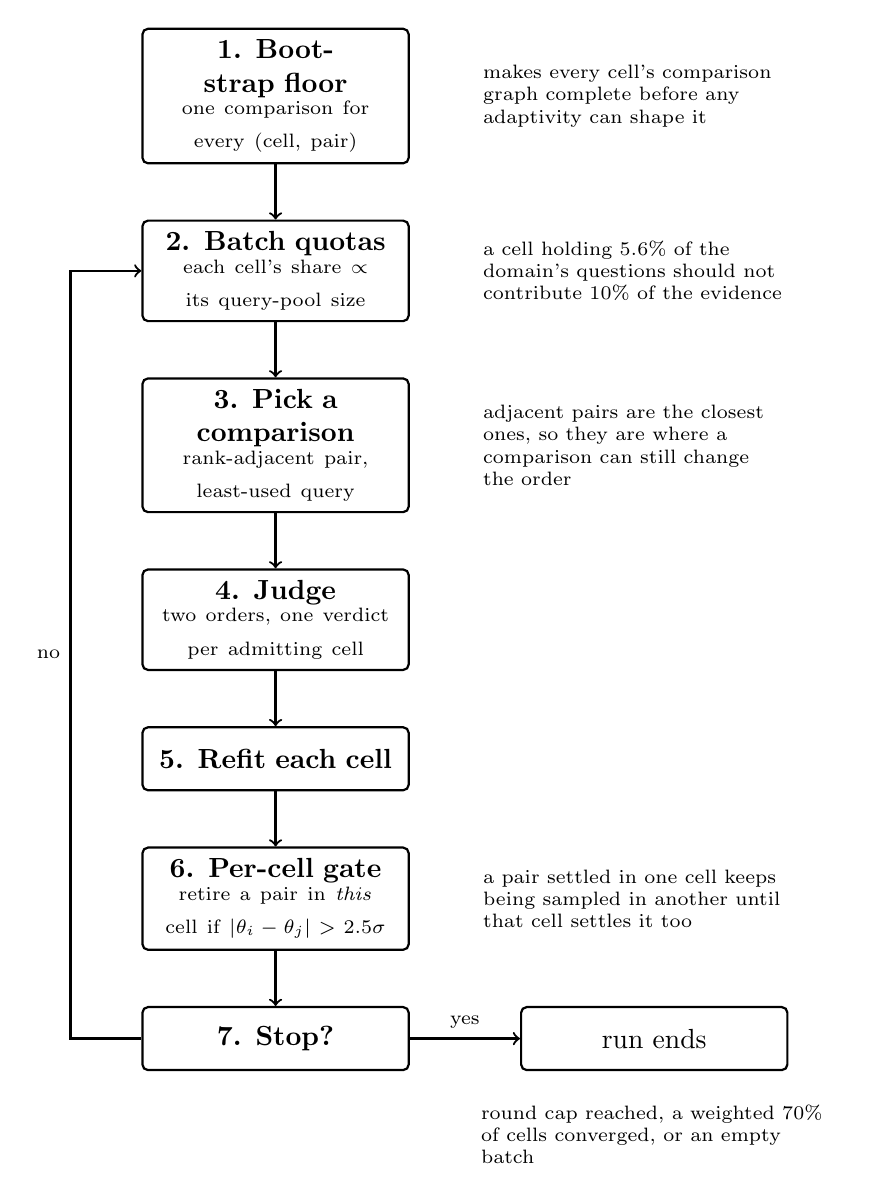
\begin{tikzpicture}[
  node distance=4mm,
  box/.style={draw, rounded corners=2pt, align=center, inner sep=4pt,
              minimum height=8mm, text width=31mm},
  small/.style={font=\scriptsize, align=left, text width=45mm},
  ->, thick
]

\node[box] (boot) {\textbf{1. Bootstrap floor}\\\scriptsize one comparison for\\\scriptsize every (cell, pair)};
\node[box, below=7mm of boot] (quota) {\textbf{2. Batch quotas}\\\scriptsize each cell's share $\propto$\\\scriptsize its query-pool size};
\node[box, below=7mm of quota] (pick) {\textbf{3. Pick a comparison}\\\scriptsize rank-adjacent pair,\\\scriptsize least-used query};
\node[box, below=7mm of pick] (judge) {\textbf{4. Judge}\\\scriptsize two orders, one verdict\\\scriptsize per admitting cell};
\node[box, below=7mm of judge] (fit) {\textbf{5. Refit each cell}};
\node[box, below=7mm of fit] (gate) {\textbf{6. Per-cell gate}\\\scriptsize retire a pair in \emph{this}\\\scriptsize cell if $|\theta_i-\theta_j| > 2.5\sigma$};
\node[box, below=7mm of gate] (stop) {\textbf{7. Stop?}};

\foreach \a/\b in {boot/quota, quota/pick, pick/judge, judge/fit, fit/gate, gate/stop}
  \draw (\a) -- (\b);

\draw (stop.west) -- ++(-9mm,0) |- node[pos=0.25, left, font=\scriptsize] {no} (quota.west);

\node[box, right=14mm of stop] (end) {run ends};
\draw (stop) -- node[above, font=\scriptsize] {yes} (end);

\node[small, right=8mm of boot]  {makes every cell's comparison\\graph complete before any\\adaptivity can shape it};
\node[small, right=8mm of quota] {a cell holding $5.6\%$ of the\\domain's questions should not\\contribute $10\%$ of the evidence};
\node[small, right=8mm of pick]  {adjacent pairs are the closest\\ones, so they are where a\\comparison can still change\\the order};
\node[small, right=8mm of gate]  {a pair settled in one cell keeps\\being sampled in another until\\that cell settles it too};
\node[small, below=3mm of end, text width=44mm]
  {round cap reached, a weighted $70\%$\\of cells converged, or an empty batch};

\end{tikzpicture}
\caption[The scheduling loop]{One round of the arena. The bootstrap
completes before any adaptive step and does not repeat; a pair is
terminal inside a cell by binomial significance, exhausted budget, or
the confidence gate (full rules in
Appendix~\ref{sec:app-scheduler})}
\label{fig:scheduling}
\end{figure}

The loop's full mechanics --- the per-(cell, pair) bootstrap floor,
pool-proportional batch quotas, adjacent-pair and least-used-query
selection, and the three conditions under which a pair or a run is
terminal --- are specified in Appendix~\ref{sec:app-scheduler},
together with the earlier rules they replaced and what those did to
one run.

Two properties of the scheduler bear on how results must be read.
First, \textbf{it over-samples uncertain pairs}, so mid-ranked models
face harder average opposition than a uniform design would give them.
Win-rate ignores opponent strength and is therefore biased by this;
Bradley--Terry $\theta$ is not, and Chapter~\ref{ch:results} quotes
$\theta$ throughout. Second, \textbf{the generic arm is stopped
at the cell-scoped arm's comparison count} rather than run to its own
convergence rule. An arm with less evidence has a noisier fit and a
depressed $\rho$, so any difference in arm size biases the contrast
toward whichever arm got more data. Matching the counts removes the
threat by construction.

\subsection{Bradley--Terry Estimation}\label{sec:meth-bt}

Nothing in this subsection is new. The model, the estimator, the tie
handling and the prior are standard choices taken from the
Bradley--Terry literature, and they are stated here because the
numbers they produce are read closely later, and because two of them
have to be defined before the standard errors below make sense.

The Bradley--Terry model assigns each model $m_i$ a latent strength
$s_i$ with $P(m_i \succ m_j) = \sigma(s_i - s_j)$
\parencite{bradley1952rank}. Only differences of strengths are
observable, so the zero-sum constraint $\sum_i s_i = 0$ is imposed to
fix the one degree of freedom the data cannot see; it is re-enforced
after every update sweep.
Ties contribute a half-win to each side, so $W_{ij} + W_{ji} = N_{ij}$
and a draw needs no parameter of its own. The alternative would be a
Davidson tie-propensity term, an extension of Bradley--Terry that gives
draws their own fitted parameter \parencite{davidson1970ties}. It is not fitted here. The cost of
that choice is measured rather than assumed: rule~D5 of
Section~\ref{sec:meth-discipline} exists because how a tie is scored
moves Spearman $\rho$ by a visible amount, which is why every $\rho$ in
this thesis is reported under both conventions.

The estimator is the Minorisation--Maximisation update of
\textcite{hunter2004mm}, regularised by a Jeffreys
$\mathrm{Beta}(0.5, 0.5)$ prior applied only to pairs that already
carry at least one real comparison, so the prior keeps swept pairs
finite without manufacturing edges in the comparison graph, and the
identifiability check runs on the observed counts alone. The update
rule, stopping tolerance, and the prior's exact application are set
out in Appendix~\ref{app:numerics}.

\paragraph{Per-cell standard errors.}
$\hat{\sigma}_i = \sqrt{[\mathcal{I}(\hat{\mathbf{s}})^{-1}]_{ii}}$ is
taken from the full observed Fisher information. The zero-sum
constraint makes $\mathcal{I}$ rank-deficient by one, and the
implementation does not use a pseudoinverse: it inverts the
rank-completed matrix $\mathcal{I} + \mathbf{1}\mathbf{1}^{\!\top}$ and
then removes the completion term, which requires subtracting $1/K^{2}$
from each diagonal entry. A variance floor of $10^{-6}$ and a standard
error floor of $0.01$ are applied, the second of which binds first.

\textbf{One correction, and what it left behind.}
The implementation subtracted $1/K$ rather than $1/K^{2}$, since
fixed; no pre-fix standard error is a measurement. The consequence:
\textbf{no Bradley--Terry confidence interval appears anywhere in
this thesis} --- every bracketed range reported is an interquartile
range and says so. Derivation and damage census:
Appendix~\ref{app:numerics} and the debt register
(Section~\ref{sec:disc-debt}).

\paragraph{Identifiability.}
Bradley--Terry parameters are identified only up to an additive
constant per connected component of the comparison graph, so a cell
whose graph is disconnected yields incomparable sub-scales. The
per-(cell, pair) bootstrap of Section~\ref{sec:meth-scheduling} is what
addresses this: one comparison per pair per cell makes each cell's
graph complete, which is a stronger condition than connected. The
guarantee holds only for cells the bootstrap reached; a cell whose
held-out pool is empty is excluded from the run.

\subsection{Aggregation to Domains}\label{sec:meth-aggregation}

Domain-level rankings pool cell-level sufficient statistics and refit,
\[
W_{ij,D_k} = \sum_{L \in \mathcal{D}(D_k)} W_{ij}^{(L)},
\qquad
N_{ij,D_k} = \sum_{L \in \mathcal{D}(D_k)} N_{ij}^{(L)},
\]
followed by a single fresh MM fit.
Cell-level parameters are never averaged. Bradley--Terry identification
is fixed only up to a per-component additive constant, so averaging
differently normalised cell scales produces no interpretable quantity,
whereas pooling counts and refitting yields a single shared scale. The
cell-average ranking is still computed, but only as a diagnostic that
logs a warning when it disagrees with the pooled order.

Two cells are excluded from the pool. A cell with fewer than five total
comparisons is dropped, and so is a cell where the judge agreed with
the answer key on under half of the decidable matches it saw.

The domain-level standard error is an inverse-variance combination of
the per-cell Fisher standard errors,
\[
\mathrm{SE}_{i,D_k} \;=\;
\Big(\textstyle\sum_{L \in \mathcal{D}(D_k)} \hat{\sigma}_{i,L}^{-2}\Big)^{-1/2},
\]
clamped to $[10^{-3}, 10]$. This replaced a query-level bootstrap that
resampled the domain's queries and refitted. The bootstrap was not
producing a usable number: on the mathematics re-run it returned
$0.0010$ for all twelve models against $0.4642$ from the
inverse-variance combination, a factor of $464$, and its own guard
marked every run unreliable as a result.
The replacement has a known bias and it goes the wrong way for comfort.
Inverse-variance pooling assumes the cell-level estimates are
independent. They are not, because multi-membership puts the same query
in several cells, so $\mathrm{SE}_{i,D_k}$ is a \emph{lower bound} on
the true uncertainty. It is used to order and to gate, never to print
an interval.

Pooling has a consequence for the partition comparison of
Section~\ref{sec:res-c5} that must be stated where a reader will see
it: under pooling, the partition affects only \emph{which rubric judged
each verdict}, not how the verdicts combine. The two arms of that
comparison are identical in estimation by construction, so any
difference between them is attributable to the rubric rather than to
the roll-up.

\paragraph{Mechanisms with no implementation.}\label{sec:meth-not-implemented}
Several mechanisms described in earlier design documents for this
system --- per-pair and per-cell state machines, a global escape valve,
fractional multi-cell weighting, and five others --- have no
implementation. None is load-bearing: every result in
Chapter~\ref{ch:results} was produced by the system as described above
and would be unchanged if these mechanisms were deleted from the design
documents. They are named because the design documents are part of this
project's record, and a reader comparing them against the running
system would otherwise have to work out which parts were built.
Appendix~\ref{app:not-implemented} inventories them.

\section{Validation Against the Answer Key}\label{sec:meth-validation}

Ground-truth per-domain accuracy
$A_{i,D_k} = |\{q \in Q_{D_k} : m_i(q) = y_q^{\text{MMLU}}\}| /
|Q_{D_k}|$
is computed strictly after every verdict has been recorded and is used
only for external, post-hoc validation. $Q_{D_k}$ is the set of
held-out questions whose primary cell lies under the domain's anchor,
so it is a partition of the judged set even though the cells inside a
domain overlap.

Two statistics are reported against it.

The \emph{primary} judge-side statistic is per-verdict agreement
between the judge's winner and the answer key, counted only on
\emph{decidable} matches --- those where exactly one of the two models
answered correctly. When both are right or both are wrong the key says
``tie'', which is the key declining to rank rather than a judgement
about response quality. Counting those as agreement checks scores the
judge against a reference that mostly abstains, and pins the
exact-match rate near $0.45$ regardless of how good the judge is. On
decidable matches the statistic is what it claims to be: the rate at
which the judge picks the model that actually answered correctly. It is
a proportion over thousands of verdicts.
% RESOLVED 2026-07-31: the exported agreement path (judgeAccuracyAgreement)
% now records decidable comparisons only; verified against an independent
% recomputation on a re-run of philosophy (0.7520 == 0.7520).

The \emph{secondary} statistic is Spearman $\rho$ between the fitted
$\boldsymbol{\theta}$ and $\mathbf{A}$, which is a rank correlation
over the model count and is therefore heavily quantised. The grid
derivation and the reporting rules that follow from it, including the
requirement that every $\rho$ be reported under both tie conventions,
are in Section~\ref{sec:exp-metrics}.

\section{Methodological Assumptions}\label{sec:meth-assumptions}

The method rests on six assumptions --- directional geometry as
semantic compatibility, one directional component per node, local
Bradley--Terry transitivity inside a cell, judge reliability under
domain conditioning, distinct true model rankings across cells, and
independence of comparisons given the Bradley--Terry parameters.
Table~\ref{tab:meth-assumptions} (Appendix~\ref{app:numerics})
tabulates each with the failure mode that would break it and the
diagnostic that would show it.

Three of these are load-bearing, and none of the three survived intact.
The judge-reliability assumption is the one RQ1 is about, and
Section~\ref{sec:res-judge} reports what the judge actually conditions
on. The assumption that cells carry different true rankings is the
premise of the original second research question, and
Section~\ref{sec:res-granularity} reports it as refused under
pre-registration. The independence assumption is violated and nothing
in this thesis corrects for it. The Fisher standard errors are
optimistic by an unmeasured margin, and the inverse-variance
combination that produces the domain-level figure inherits the same
optimism. This costs little in practice, because the headline quantity
is a paired contrast and no interval is reported.

\section{Measurement Discipline}\label{sec:meth-discipline}

This section states five rules about how a measurement in this thesis
must be produced and reported. They are not general methodological
advice. Each one is here because this project broke it at least once,
got a wrong answer, and only then wrote the rule down, so each is given
together with the failure that produced it. A rule stated with the
error behind it can be checked; a rule stated as foresight has to be
taken on trust. And Chapter~\ref{ch:results} reports several nulls, and
a null carries information only if the reader knows what would have
counted as an effect.

\textbf{D1 --- A test that cannot fail is not a test.}
Before running a check, ask what result would falsify it; if the answer
is ``none available'', a clean result carries no information.
Instance: the corpus validator's \texttt{TRACE\_PRESENCE} check has no
failure branch at all, and six of the ten hard-excluded models are
excluded for exactly the condition it measures and declines to act on
(the full policy story is Section~\ref{sec:exp-rosters}).
% MOVED-CANDIDATE (D1, second instance; was a footnote here --
% relocate to the corrections register): A second instance: an audit
% that classified every identifier column by set membership against
% every known identifier space returned approximately $100\%$
% everywhere, because these are dense small-integer ranges over one
% corpus. The spaces coincide as sets while disagreeing about which row
% each value points to.

\textbf{D2 --- Report a join's overlap before reporting the join's
result.}
A join with little key overlap produces a clean-looking null
indistinguishable from a real one, so any analysis concluding ``no
effect'' must first report the number of join groups that could have
shown an effect.
Instance, and the one that reached the results: the corpus's
\texttt{mmlu\_pro.id} is not the evaluation table's
\texttt{question\_id}. The numeric join between them succeeds, returns
well-formed rows, and is wrong. It is what collapsed the law domain
from 287 questions to 20 and inverted a domain recommendation
(Section~\ref{sec:res-law}). Joins in this project go through query
text.
% MOVED-CANDIDATE (D2, second instance; was a footnote here --
% relocate to the corrections register): An earlier instance: a design
% change was made on measured evidence of ``0 of 36 rescues''. The join
% was on an iteration counter that one code path hardcoded to $-1$, so
% the numerator was structurally impossible; the mixed-group count was
% $0$ of $613$ before the defect was fixed and $97$ of $613$ after ---
% a single figure that would have caught it at no cost. The corrected
% join gives 3 rescues in 404, and a subsequent run refuted the change.

\textbf{D3 --- Report a median with its interquartile range, and claim
only what the spread supports.}
Instance: $\mathrm{SE}(\Delta J)$ varies by more than an order of
magnitude across sites on this corpus
(Section~\ref{sec:res-construction}), which is the entire reason the
acceptance gate is expressed in standard-error units.
% MOVED-CANDIDATE (D3, second instance; was inline here -- relocate to
% the corrections register): Instance: the acceptance gate's apparent
% dispersion degradation --- a coefficient of variation that rose
% mechanically because the mean fell, initially read as a real change
% --- which dissolves under this rule; the full statistical reading is
% reported with the result (Section~\ref{sec:res-construction}).

\textbf{D4 --- A threshold derived for one quantity at one stage does
not transfer.}
Instance: a single separation constant served split acceptance,
component selection, sibling merging and the global proposal gate;
because one of those gates weights its divergence by the fitted
concentration, the same constant meant about $8.1^{\circ}$ of angular
tolerance at freshly split nodes and under $0.7^{\circ}$ at deep
ones, which is why it almost never fired.
% MOVED-CANDIDATE (D4, second and third instances; was a footnote here
% -- relocate to the corrections register): Two further instances. A
% second constant served both as a \emph{level} (``is this partition
% separated at all?'') and as a \emph{difference} (``does one more
% cluster buy enough over the last?''); these are different quantities
% and were decoupled into separate fields. A third, a float tolerance,
% serves simultaneously as a per-edit acceptance band and as a
% per-iteration fixed-point tolerance; the acceptance half has since
% been replaced by the standard-error gate, and the certificate half
% still borrows a constant derived for the other question.

\textbf{D5 --- Report a rank correlation under both tie conventions.}
This rule is newer than the other four and was forced by the results of
Section~\ref{sec:res-tie-policy}. Half-weighting ties and dropping tied
comparisons are both defensible, and on the same verdict set they move
Spearman $\rho$ by up to $\pm0.029$ in a direction that is not
consistent across conditions. On one paired contrast the two
conventions disagree about which arm is ahead by more than the
registered decisive threshold. That threshold has since been withdrawn
(Section~\ref{sec:exp-metrics}), and the observation survives it: a
single $\rho$ from this pipeline is not a result.

\section{Persistence and Reproducibility}\label{sec:arch-infra}

\textbf{What the seed does.}
A run takes one integer. It is the only randomness the pipeline takes
from outside itself --- wherever else a shuffle or a sample appears,
its generator is keyed off the data it is shuffling and is therefore
fixed once the data is --- and it drives two things.
First, the split: the corpus is shuffled inside each of the 14
MMLU-Pro categories and cut $70/30$, so the seed decides which
questions the construction and the rubrics are allowed to see and which
are held out for judging.
Second, arena scheduling: the offsets the bootstrap phase walks across
each cell's query pool.
Everything between those two points is deterministic. The directional
fits at each candidate split have no random initialisation, and the
acceptance gates are arithmetic on the fitted quantities, so a fixed
seed and a fixed commit rebuild the same tree --- the same node and
cell counts, the same queries in the same cells, and the same accepted
separations. That is what ``reproducible'' means here, and it has been
checked rather than assumed: a rebuild from the same configuration
reproduced the then-frozen artifact's cell partition exactly, and all
50 of its accepted-split separations to nine decimal places.
The claim stops at the partition. Two fields of the fixed-point
certificate move in the last few digits between two runs of the same
commit at the same seed, because routing is parallel and floating-point
addition is not associative; they are bounded rather than
bit-identical.

What the seed does \emph{not} do is make a result seed-independent. It
fixes which of the possible constructions the thesis is talking about;
it says nothing about whether a different draw would have given a
different one. The run-to-run spread that leaves is a real limitation
and is reported under R3 (Section~\ref{sec:res-construction}). Every
construction and arena result in this thesis is at seed 42.

Any result is specified by the tuple
\texttt{(corpusVersion, snapshotId, runId)}; the four SQLite stores
this rests on, and the run manifest with its two qualifications (a
working-tree flag that fires on benign conditions, and a ratings store
whose re-runs clear rather than accumulate), are described in
Appendix~\ref{sec:num-persistence}.
